\documentclass[aip,jcp,reprint,noshowkeys,superscriptaddress]{revtex4-1}
\usepackage{graphicx,dcolumn,bm,xcolor,microtype,multirow,amscd,amsmath,amssymb,amsfonts,physics,wrapfig,txfonts,siunitx}
\usepackage[version=4]{mhchem}
%\usepackage{natbib}
\bibliographystyle{achemso}

\newcommand{\ie}{\textit{i.e.}}
\newcommand{\eg}{\textit{e.g.}}
\newcommand{\alert}[1]{\textcolor{black}{#1}}
\usepackage[normalem]{ulem}
\newcommand{\fk}[1]{\textcolor{blue}{#1}}
\newcommand{\titou}[1]{\textcolor{red}{#1}}
\newcommand{\trashPFL}[1]{\textcolor{red}{\sout{#1}}}
\newcommand{\PFL}[1]{\titou{(\underline{\bf PFL}: #1)}}
\newcommand{\toto}[1]{\textcolor{green}{#1}}
\newcommand{\trashAS}[1]{\textcolor{green}{\sout{#1}}}
\newcommand{\AS}[1]{\toto{(\underline{\bf AS}: #1)}}
\newcommand{\ant}[1]{\textcolor{orange}{#1}}
\newcommand{\SupInf}{\textcolor{blue}{Supporting Information}}

\newcommand{\mc}{\multicolumn}
\newcommand{\fnm}{\footnotemark}
\newcommand{\fnt}{\footnotetext}
\newcommand{\tabc}[1]{\multicolumn{1}{c}{#1}}
\newcommand{\QP}{\textsc{quantum package}}

\newcommand{\EHF}{E_\text{HF}}
\newcommand{\EDOCI}{E_\text{DOCI}}
\newcommand{\EFCI}{E_\text{FCI}}
\newcommand{\Ndet}{N_\text{det}}
\newcommand{\Nbas}{N}

\usepackage[
	colorlinks=true,
    citecolor=blue,
    breaklinks=true
	]{hyperref}
\urlstyle{same}

\begin{document}

\newcommand{\LCPQ}{Laboratoire de Chimie et Physique Quantiques (UMR 5626), Universit\'e de Toulouse, CNRS, UPS, France}

\title{Seniority and hierarchy configuration interaction for radicals and excited states}

\author{F\'abris Kossoski}
\email{fkossoski@irsamc.ups-tlse.fr}
\affiliation{\LCPQ}
\author{Pierre-Fran\c{c}ois Loos}
\email{loos@irsamc.ups-tlse.fr}
\affiliation{\LCPQ}

% Abstract
\begin{abstract}
{\bf Abstract:} 
%\bigskip
%\begin{center}
%        \boxed{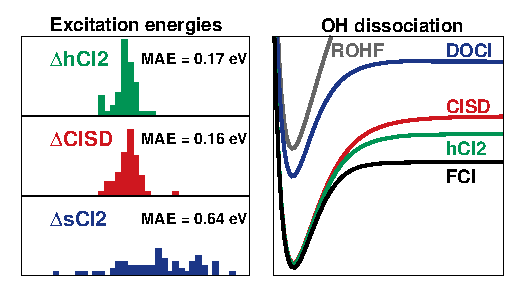
\includegraphics[keepaspectratio,width=2in]{TOC}}
%\end{center}
%\bigskip
\end{abstract}

% Title
\maketitle


%%%%%%%%%%%%%%%%%%%%%%%%%%%%%%%%%%%%%%%%%%%%%%%%%%
\section{Introduction}
\label{sec:intro}
%%%%%%%%%%%%%%%%%%%%%%%%%%%%%%%%%%%%%%%%%%%%%%%%%%


Seniority based methods.
Limited studies for radicals and excited states

Hierarchy CI \cite{Kossoski_2022}
Similarly, only for closed-shell systems.

We introduce single-reference CI approximations built on top of an open-shell reference.
Seniority and hCI.
How do these methods perform for ground state radicals?
Impact of perturbative correction.

Ground-state based CI vs. state-specific CI \cite{Kossoski_2023}
Promising results for state-specific excitation-based CI.
We introduce analogous state-specific seniority-based CI ($\Delta$sCI) and hierarchy-based CI ($\Delta$hCI).
$\Delta$sCI2 
$\Delta$hCI1
How do these methods perform for excited states, from both closed-shell and open-shell systems?



%For an arbitrary reference Slater determinant, with seniority $s_0$, the hierarchy $h$ associated to a another determinant
With respect to a given reference Slater determinant, the hierarchy $h$ of a target determinant is defined as
\begin{equation}
        \label{eq:h}
        %h = \frac{e+\Delta s/2}{2},
	h = \frac{e+ (s-s_0)/2}{2},
\end{equation}
where $s$ and $s_0$ denote the seniority of target and reference determinants, respectively, and $e$ represents the excitation degree that connect the two determinants.
This definition renders a degree of dissimilarity between two determinants (reference and target),
which accounts for differences in orbital occupation (through the excitation degree $e$)
and differences in the number of unpaired electrons (through the term $(s-s_0)/2$).
The latter always assumes an integer value (for both even and odd numbers of electrons), such that $h$ becomes an integer or half-integer.
Also, Eq.~\eqref{eq:h} simplifies to the previous definition \cite{Kossoski_2022} for the case of a closed-shell reference determinant, when $s_0 = 0$.

%%%%%%%%%%%%%%%%%%%%%%%%%%%%%%%%%
\section{Computational details}
\label{sec:compdet}
%%%%%%%%%%%%%%%%%%%%%%%%%%%%%%%%

To gauge the performance of hCI against excitation-based and seniority-based CI for radical systems,
we have calculated the potential energy curves (PECs) for the dissociation of four radical systems:
\ce{OH}, \ce{CN}, vinyl (\ce{C2H3}), and \ce{H7}.
%which display a variable number of bond breaking.
The equilibrium geometry of vinyl was taken from Ref.~\onlinecite{Loos_2020},
%also reproduced in the \SupInf,
and the PECs were computed along the \ce{C=C} double bond breaking coordinate, with the remaining internal coordinates kept frozen.
For \ce{H7}, we considered equally spaced and linearly arranged hydrogen atoms, and the PECs were computed along the symmetric dissociation coordinate.
From the PECs, we performed a similar analysis as in our paper on hCI for closed-shell systems. \cite{Kossoski_2022}
Namely, for the different CI levels considered here, 
we evaluated the convergence of the non-parallelity error (NPE), the distance error, the vibrational frequencies, and the equilibrium geometries, as functions of $\Ndet$.
The NPE (distance error) of a given level of theory is defined as the maximum minus (plus) the minimum differences between its corresponding PEC and the FCI PEC.
Details about how the vibrational frequencies and equilibrium geometries were obtained from the calculated PECs can be found in the \SupInf.

To evaluate how the different levels of CI introduced here perform for excited states,
we calculated vertical excitation energies for 60 electronic states, comprising 26 different molecular systems, with geometries extracted from the QUEST database. \cite{Veril_2021}
% 18 closed-shells, 8 radicals
We employed the aug-cc-pVDZ basis set for systems having up to three non-hydrogen atoms and the 6-31+G(d) basis set for the larger ones.
We performed calculations following both the standard ground-state based CI route and the state-specific CI route. \cite{Kossoski_2023}
For the latter, we employed the state-specific orbitals obtained in Ref.~\onlinecite{Kossoski_2023}.
The computed excitation energies were compared against the reference values from the QUEST database. \cite{Veril_2021}
The full set of excited states and calculated excitation energies, for the various methods considered here, are provided in the {\SupInf}.
%For completeness, we also reproduce the geometries in the \SupInf.

The hCI methods introduced here were implemented in {\QP} \cite{Garniron_2019} through a straightforward modification of the
\textit{configuration interaction using a perturbative selection made iteratively} (CIPSI) algorithm. \cite{Huron_1973,Giner_2013,Giner_2015,Garniron_2018}
By allowing only for the determinants that are connected with the reference determinant(s) up to a given maximum hierarchy $h$,
the CIPSI algorithm is restricted to the truncated Hilbert space defined by the reference and the value of $h$.
{\QP} \cite{Garniron_2019} was employed to perform all the CI calculations presented here.
In a given calculation, the energies are considered to be converged when the (largest) Epstein-Nesbet second-order perturbation correction computed in the truncated Hilbert space 
lies below \SI{0.01}{\milli\hartree}. \cite{Garniron_2018}
%by spanning the most important regions of the truncated Hilbert space
This selected CI procedure requires considerably fewer determinants than the total number of determinants in the truncated Hilbert space,
while delievering fairly converged absolute and excitation energies.
The ground- and excited-state CI energies are obtained with the Davidson iterative algorithm. \cite{Davidson_1975}

%restricted open-shell HF orbitals


%%%%%%%%%%%%%%%%%%%%%%%%%%%%%%%%
\section{Results and discussion}
\label{sec:res}
%%%%%%%%%%%%%%%%%%%%%%%%%%%%%%%%


%%%%%%%%%%%%%%%%%%%%%%%%%%%%%%%%
\subsection{hCI for radicals}
\label{sec:res_A}
%%%%%%%%%%%%%%%%%%%%%%%%%%%%%%%%


PECs
NPEs, distance errors
equilibrium geometries and vibrational frequencies

HF orbitals
orbital optimization?

perturbative correction for closed- and open-shell systems


%%%%%%%%%%%%%%%%%%%%%%%%%%%%%%%%
\subsection{hCI for excited states}
\label{sec:res_B}
%%%%%%%%%%%%%%%%%%%%%%%%%%%%%%%%

hCI1/HF
hCI1.5/HF
hCI2/HF
$\Delta$hCI1
$\Delta$hCI1.5
$\Delta$hCI2

Higher-order levels for a few systems
hCI2.5/HF
hCI3/HF
$\Delta$hCI2.5
$\Delta$hCI3
$\Delta$hCI3.5

%%%%%%%%%%%%%%%%%%%%%%%%%%%%%%%%
\subsection{Seniority CI for excited states}
\label{sec:res_C}
%%%%%%%%%%%%%%%%%%%%%%%%%%%%%%%%

sCI2
$\Delta$sCI2


%%%%%%%%%%%%%%%%%%%%%%%%%%%%%%%%
\section{Conclusion}
\label{sec:ccl}
%%%%%%%%%%%%%%%%%%%%%%%%%%%%%%%%

%%%%%%%%%%%%%%%%%%%%%%%%%%%%%%%%
\begin{acknowledgements}
This work was performed using HPC resources from CALMIP (Toulouse) under allocation 2021-18005.
This project has received funding from the European Research Council (ERC) under the European Union's Horizon 2020 research and innovation programme (Grant agreement No.~863481).
\end{acknowledgements}
%%%%%%%%%%%%%%%%%%%%%%%%%%%%%%%%

%%%%%%%%%%%%%%%%%%%%%%%%%%%%%%%%%%
\section*{Supporting information available}
\label{sec:SI}
%%%%%%%%%%%%%%%%%%%%%%%%%%%%%%%%%%

%%%%%%%%%%%%%%%%%%%%%%%%%%%%%%%%
%\section*{Data availability statement}
%%%%%%%%%%%%%%%%%%%%%%%%%%%%%%%%
%The data that support the findings of this study are openly available in Zenodo at \href{http://doi.org/XX.XXXX/zenodo.XXXXXXX}{http://doi.org/XX.XXXX/zenodo.XXXXXXX}.

%%%%%%%%%%%%%%%%%%%%%%%%%%%%%%%%
\bibliography{manuscript}
%%%%%%%%%%%%%%%%%%%%%%%%%%%%%%%%

\end{document}
